\newpage
\section{Билет 16. Вязкая жидкость. Закон Навье-Стокса. Уравнения Навье-Стокса. Полная система уравнения, описывающая движение вязкой несжимаемой жидкости. Течение Пуазейля. Течение Куэтта. Закон Фурье. Полная система уравнений, описывающая движение вязкого теплопроводного совершенного газа.}

\begin{center}
	\textit{\underline{Вязкая жидкость}}
\end{center}

\begin{defn}
	Жидкость или газ называются \textbf{вязкими}, если в них при движении, возможно касательные напряжения. В таком случае компоненты тензора напряжений в вязкой жидкости представляются в виде: $$p^{ij}=-pg^{ij} + \tau^{ij},  \tau^{ij} = \tau^{ij}(e_{kl}, T) ,$$
	где $p$-давление, $e_kl$ - компоненты тензора скоростей деформаций, $T$-температура. 
\end{defn}

\begin{defn}
	\textbf{Компонентами тензора вязких напряжений} называются $\tau^{ij}$.
\end{defn}

Заметим, что если жидкость покоится, то $\tau^{ij} = 0$.

\begin{defn}
	Жидкость или газ называются \textbf{линейно-вязкими (или ньютоновскими)}, если $\tau^{ij}$ являются линейными функциями компонент тензора скоростей деформации ($e_{kl}$), т.е.: $$\tau^{ij} = A^{ijkl}e_{kl}, $$ где $A^{ijkl}$-коэффиценты вязкости.
\end{defn}


Ньютон в своем опыте с двумя пластинами выявил такую характеристику жидкости или газа, как вязкость.  Это свойство жидкости проявляется лишь при ее движении. Допустим, что некоторое количество жидкости заключено между двумя плоскими неограниченными параллельными пластинами; расстояние между ними – $d$; скорость движения верхней пластины относительно нижней – $v_0$.

Опыт показывает, что слой жидкости, непосредственно прилегающий к стенке, прилипает к ней. Отсюда следует, что скорость движения жидкости, прилегающей к нижней стенке, равна нулю, а к верхней – $v_0$. Промежуточные слои движутся со скоростью, постепенно возрастающей от $0$ до $v_0$.

Чтобы перемещать одну пластину относительно другой, необходимо приложить к движущейся пластине некоторую силу $F$, равную силе сопротивления жидкости в результате внутреннего трения. Ньютон установил, что эта сила пропорциональна скорости $v_0$, поверхности соприкосновения $S$ и обратно пропорциональна расстоянию между пластинами $d$ т.е.:
$$F = \mu\frac{S v_0}{d}$$

\begin{figure}[H]
	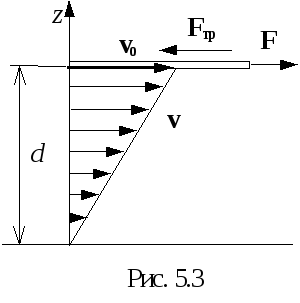
\includegraphics[width=0.4\textwidth]{16/newton_experiment.png}
\end{figure}


\begin{center}
	\textit{\underline{Закон Навье-Стокса}}
\end{center}


\begin{defn}
	\textbf{Изотропность} - совпадение свойства по всем направлениям. 
\end{defn}

\begin{theorem}[Э-132]Закон Навье-Стокса
	Для изотропных, линейно-вязких жидкостей верно следующее утверждение:
	$$\tau^{ij} = \lambda I_1(e)g^{ij}+2\mu e^{ij},$$ где $\lambda$, $\mu$ - коэффиценты вязкости, $I_1(e) = e_{ij}g^{ij}$ - первый инвариант тензора скоростей деформаций.
\end{theorem}


\begin{center}
	\textit{\underline{Уравнения Навье-Стокса}}
\end{center}

Уравнения движения линейно-вязких жикостей или газов называется уравнением Навье-Стокса. Они получаются из универсальных газовых уравнений: $$\rho\frac{dv^i}{dt} = \rho F^i + \nabla_{i}p^{ij}$$ подстановкой выражений для $p^{ij}$ и $\tau^{ij}$ и выведением уравнений покомпонентно.

Итоговое уравнение Навью-Стокса:

$$\frac{dv}{dt} = \hat{F} - \frac{1}{\rho}grad p + \frac{\lambda + \mu}{\rho}grad(div \hat{v}) + \frac{\mu}{\rho}\Delta \hat{v}$$


\begin{center}
	\textit{\underline{Полная система уравнения, описывающая движение вязкой несжимаемой жидкости}}
\end{center}


Полна система механических уравнений для несжимаемой линейно-вязкой жидкости с постоянными коэффицентами вязкости состоит из уравнения неразрывности, условия несжимаемости и уравнения Навье-Стокса:

\begin{equation} \label{eq:task}
	\begin{cases}
		\begin{array}{l}
			div \, \hat{v} = 0\\
			\frac{d\rho}{dt} = \frac{\partial \rho}{\partial t} + v^k\frac{\partial \rho}{\partial x^k} = 0\\
			\frac{dv}{dt} = \hat{F} - \frac{1}{\rho}grad\, p + \frac{\mu}{\rho}\Delta \hat{v}
		\end{array}
	\end{cases}
\end{equation}

\begin{center}
	\textit{\underline{Течение Пуазейля}}
\end{center}

\begin{defn}
	\textbf{Течение Пуазейля} - ламинарное течение жидкости через каналы в виде прямого кругового цилиндра или слоя между параллельными плоскостями. Течение Пуазёйля — одно из самых простых точных решений уравнений Навье — Стокса. Описывается законом Пуазёйля (также называемым законом Гагена — Пуазёйля или Хагена — Пуазёйля).
\end{defn}

\begin{figure}[H]
	\centering
	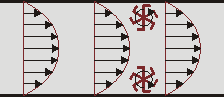
\includegraphics[width=0.4\textwidth]{16/poiseuille_profile.png}
\end{figure}

Течение Пуазёйля характеризуется параболическим распределением скорости по радиусу трубки. В каждом поперечном сечении трубки средняя скорость вдвое меньше максимальной скорости в этом сечении.


\begin{center}
	\textit{\underline{Течение Куэтта}}
\end{center}

\begin{defn}
	\textbf{Течение Куэтта} - ламинарное течение вязкой жидкости между двумя параллельными стенками (не обязательно прямолинейными), одна из которых двигается относительно другой. Течение происходит под действием сил вязкого трения, действующих на жидкость, и сдвигового напряжения параллельного стенкам.
\end{defn}


